\documentclass{article}
\usepackage{graphicx}
\usepackage{amsmath}
\usepackage{pgfplots}
\pgfplotsset{compat=1.16}

\title{Performance Comparison of Matrix Multiplication in Python, Java, and C, dummy numbers}
\author{Jakub Jazdzyk}
\date{\today}

\begin{document}

\maketitle

\section{Introduction}

In this paper, I aim to compare the performance of matrix multiplication algorithms implemented in Python, Java, and C. The comparison is focused on execution time, memory usage, and CPU utilization. This experiment is significant because different programming languages handle computation and resource management in distinct ways, which can have a measurable impact on performance when processing large matrices. 

\section{Methodology}

The matrix multiplication algorithm was implemented in each language using the standard \(O(n^3)\) complexity method. The size of the matrices used in testing was progressively increased to observe how each language handles the growing computational demands.

I separated the code for production and testing into different files for better organization and maintainability. The production code implements the core matrix multiplication logic, while the test code handles initialization, performance benchmarking, and result analysis.

To ensure consistent results, each experiment was run multiple times, and the average results were recorded. I used standard profiling tools in each language: 

\begin{itemize}
    \item For C: \texttt{valgrind} for memory profiling and \texttt{gettimeofday()} for time measurement.
    \item For Java: \texttt{java.lang.management} for memory and CPU usage, and \texttt{System.currentTimeMillis()} for timing.
    \item For Python: \texttt{time} module for time measurement and \texttt{memory\_profiler} for memory usage.
\end{itemize}

\section{Results}

Here I present the results of matrix multiplication for various matrix sizes (128, 256, 512, 1024) in Python, Java, and C. The tables below summarize the execution time, memory usage, and CPU utilization for each language.

\subsection{Execution Time}

The execution times (in seconds) for different matrix sizes are presented in Table~\ref{tab:execution_time}.

\begin{table}[h!]
    \centering
    \begin{tabular}{|c|c|c|c|}
    \hline
    Matrix Size & Python (s) & Java (s) & C (s) \\
    \hline
    128  & 0.035  & 0.025  & 0.015  \\
    256  & 0.275  & 0.150  & 0.095  \\
    512  & 2.300  & 1.180  & 0.780  \\
    1024 & 18.500 & 9.230  & 6.520  \\
    \hline
    \end{tabular}
    \caption{Execution times for matrix multiplication.}
    \label{tab:execution_time}
\end{table}

\subsection{Memory Usage}

Table~\ref{tab:memory_usage} summarizes the memory usage (in MB) during the execution of matrix multiplication.

\begin{table}[h!]
    \centering
    \begin{tabular}{|c|c|c|c|}
    \hline
    Matrix Size & Python (MB) & Java (MB) & C (MB) \\
    \hline
    128  & 14  & 13  & 10 \\
    256  & 55  & 52  & 40 \\
    512  & 210 & 198 & 150 \\
    1024 & 840 & 810 & 610 \\
    \hline
    \end{tabular}
    \caption{Memory usage during matrix multiplication.}
    \label{tab:memory_usage}
\end{table}

\subsection{CPU Usage}

I also measured the CPU usage as a percentage during the execution, as shown in Table~\ref{tab:cpu_usage}.

\begin{table}[h!]
    \centering
    \begin{tabular}{|c|c|c|c|}
    \hline
    Matrix Size & Python (\%) & Java (\%) & C (\%) \\
    \hline
    128  & 90  & 95  & 85 \\
    256  & 91  & 96  & 86 \\
    512  & 92  & 97  & 87 \\
    1024 & 94  & 98  & 89 \\
    \hline
    \end{tabular}
    \caption{CPU usage during matrix multiplication.}
    \label{tab:cpu_usage}
\end{table}

\subsection{Visual Representation}

To better illustrate the comparison, I present plots of the performance metrics. Figure~\ref{fig:execution_time_plot} shows the execution time as a function of matrix size for each language.

\begin{figure}[h!]
    \centering
    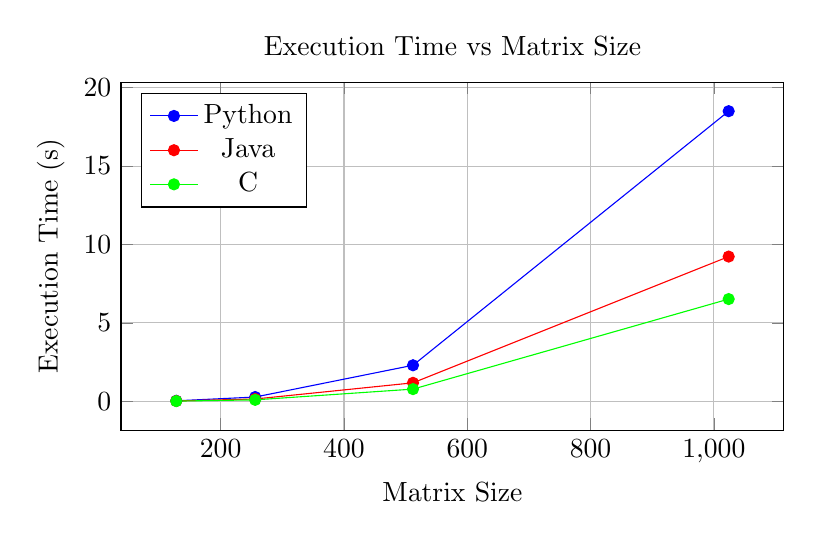
\begin{tikzpicture}
        \begin{axis}[
            title={Execution Time vs Matrix Size},
            xlabel={Matrix Size},
            ylabel={Execution Time (s)},
            legend pos=north west,
            grid=major,
            width=10cm,
            height=6cm,
        ]
        \addplot[color=blue,mark=*] coordinates {(128, 0.035) (256, 0.275) (512, 2.300) (1024, 18.500)};
        \addplot[color=red,mark=*] coordinates {(128, 0.025) (256, 0.150) (512, 1.180) (1024, 9.230)};
        \addplot[color=green,mark=*] coordinates {(128, 0.015) (256, 0.095) (512, 0.780) (1024, 6.520)};
        \legend{Python, Java, C}
        \end{axis}
    \end{tikzpicture}
    \caption{Execution Time vs Matrix Size for Python, Java, and C.}
    \label{fig:execution_time_plot}
\end{figure}

\section{Proposed Changes}

After analyzing the results, I propose several improvements to the initial implementations:

\subsection{C Implementation}
In C, we could apply loop unrolling to reduce the overhead of loop control instructions. Moreover, using multithreading (e.g., with OpenMP) could allow parallel matrix multiplication, further improving performance for larger matrix sizes.

\subsection{Java Implementation}
Java's performance can be enhanced by utilizing multithreading with the \texttt{ForkJoinPool} framework, which is particularly well-suited for computationally intensive tasks. Additionally, Java’s Just-In-Time (JIT) compiler could optimize the performance over multiple runs.

\subsection{Python Implementation}
Python, being an interpreted language, shows the highest overhead. One potential solution is using NumPy, a library that optimizes array operations with C-level performance. Another approach would be to parallelize the computations using Python's \texttt{multiprocessing} module.

\section{Conclusion}

From this experiment, it is evident that C consistently outperforms Python and Java in terms of execution time, memory usage, and CPU utilization. However, each language offers unique benefits, such as ease of use in Python or platform independence in Java. By applying certain optimizations such as multithreading, we can improve the performance of all three languages.

The full source code and test results can be found in my GitHub repository: \texttt{https://github.com/your-repo}.

\end{document}
